\chapter{Resultados de la simulaci\'on y discusi\'on termoecon\'omica}
\label{chap:resultados}

Este cap\'itulo presenta el an\'alisis cuantitativo de los resultados obtenidos a partir de la simulaci\'on de tres a\~nos completos ($2023-2025$, equivalentes a $26.280\text{ horas}$) del comportamiento de enfriamiento de un rack de Inteligencia Artificial de alta densidad ($100\text{ kW}$) en seis ubicaciones globales estrat\'egicas \cite{masnet2020}.

\section{An\'alisis del potencial de free cooling (FCP \%)}
La efectividad del Free Cooling se mide mediante el porcentaje de Horas de Free Cooling (FCP, \emph{Free Cooling Percentage}), el cual representa la fracci\'on de tiempo en la cual el sistema disipa la totalidad de la carga t\'ermica de $100\text{ kW}$ de manera puramente pasiva (sin compresi\'on de vapor mec\'anica) \cite{greengrid2008}.
\begin{equation}
FCP = \left( \frac{\sum_{h=1}^{H} \mathbb{I}(T_{ext, h} < T_{cr})}{H} \right) \cdot 100
\end{equation}
Donde $\mathbb{I}$ es la funci\'on indicadora y $H = 26.280\text{ horas}$.

La Tabla~\ref{tab:fcp_tesis} resume las horas y porcentajes de Free Cooling trienales por tecnolog\'ia.

\begin{table}[htbp]
\caption{Horas de Free Cooling y FCP por Tecnolog\'ia (2023--2025)}
\label{tab:fcp_tesis}
\centering
\resizebox{\textwidth}{!}{%
\begin{tabular}{lccc}
\toprule
Localidad & RDHx ($T_{cr} = 10^\circ\text{C}$) & D2C Bif\'asico ($T_{cr} = 25^\circ\text{C}$) & Inmersi\'on ($T_{cr} = 35^\circ\text{C}$) \\
\midrule
Isla Gordon, Chile & $25.378\text{ h } (96,6\%)$ & $26.280\text{ h } (100,0\%)$ & $26.280\text{ h } (100,0\%)$ \\
Reykjavik, Islandia & $21.411\text{ h } (81,5\%)$ & $26.280\text{ h } (100,0\%)$ & $26.280\text{ h } (100,0\%)$ \\
Lule\aa, Suecia & $17.498\text{ h } (66,6\%)$ & $26.155\text{ h } (99,5\%)$ & $26.280\text{ h } (100,0\%)$ \\
Helsinki, Finlandia & $15.823\text{ h } (60,2\%)$ & $26.208\text{ h } (99,7\%)$ & $26.280\text{ h } (100,0\%)$ \\
Quebec, Canad\'a & $15.195\text{ h } (57,8\%)$ & $25.467\text{ h } (96,9\%)$ & $26.280\text{ h } (100,0\%)$ \\
Colchane, Chile & $14.887\text{ h } (56,6\%)$ & $26.280\text{ h } (100,0\%)$ & $26.280\text{ h } (100,0\%)$ \\
\bottomrule
\end{tabular}%
}
\end{table}

\begin{figure}[htbp]
\centering
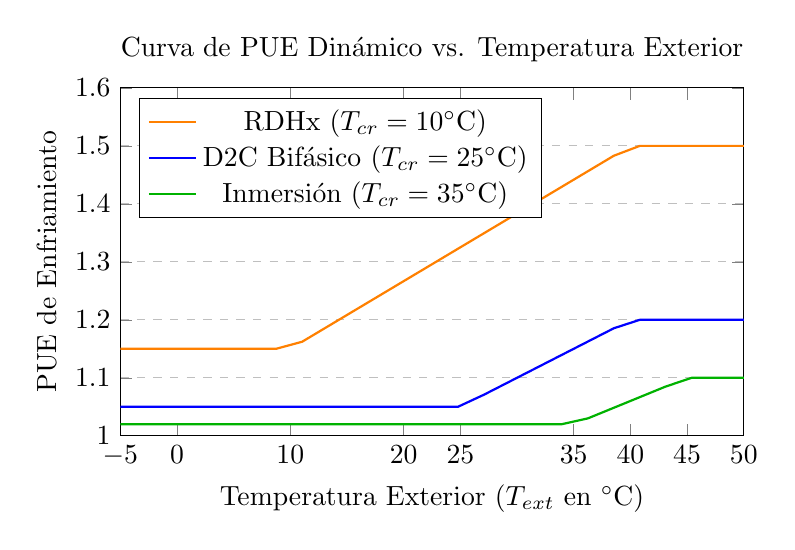
\begin{tikzpicture}
\begin{axis}[
    title={Curva de PUE Din\'amico vs. Temperatura Exterior},
    xlabel={Temperatura Exterior ($T_{\text{ext}}$ en $^\circ$C)},
    ylabel={PUE de Enfriamiento},
    xmin=-5, xmax=50,
    ymin=1.0, ymax=1.6,
    xtick={-5,0,10,20,25,35,40,45,50},
    ytick={1.0,1.1,1.2,1.3,1.4,1.5,1.6},
    legend pos=north west,
    ymajorgrids=true,
    grid style=dashed,
    width=9.5cm, height=6.0cm
]

% RDHx curve
\addplot[
    color=orange,
    thick,
    domain=-5:50,
]
{x < 10 ? 1.15 : (x > 40 ? 1.50 : 1.15 + (1.50 - 1.15) * (x - 10)/(40 - 10))};
\addlegendentry{RDHx ($T_{cr}=10^\circ$C)}

% D2C curve
\addplot[
    color=blue,
    thick,
    domain=-5:50,
]
{x < 25 ? 1.05 : (x > 40 ? 1.20 : 1.05 + (1.20 - 1.05) * (x - 25)/(40 - 25))};
\addlegendentry{D2C Bif\'asico ($T_{cr}=25^\circ$C)}

% Immersion curve
\addplot[
    color=green!70!black,
    thick,
    domain=-5:50,
]
{x < 35 ? 1.02 : (x > 45 ? 1.10 : 1.02 + (1.10 - 1.02) * (x - 35)/(45 - 35))};
\addlegendentry{Inmersi\'on ($T_{cr}=35^\circ$C)}

\end{axis}
\end{tikzpicture}
\caption{Curvas te\'oricas de transici\'on de PUE din\'amico para las tres tecnolog\'ias evaluadas (Fuente: Elaboraci\'on propia).}
\label{fig:pue_curves}
\end{figure}

Los resultados revelan que la zona austral de Chile (\textbf{Isla Gordon}) exhibe un potencial t\'ermico superior al de los centros tradicionales del hemisferio norte, superando a Lule\aa\ en un $30,0\%$ absoluto de horas de enfriamiento libre en la configuraci\'on RDHx, debido a la alta estabilidad clim\'atica patag\'onica \cite{masnet2020}. 

Por su parte, \textbf{Colchane}, ubicado en el altiplano, compensa la radiaci\'on solar diurna con bajas temperaturas nocturnas extremas, logrando un $100\%$ de FCP en D2C e Inmersi\'on \cite{bnef2024}.

\section{Evaluaci\'on termoecon\'omica (OPEX acumulado)}
El costo de operaci\'on de energ\'ia ($OPEX$) se deriva del consumo del rack de TI y de la infraestructura de enfriamiento asociada, integrando el PUE din\'amico obtenido hora a hora \cite{greengrid2008}:
\begin{equation}\label{eq:opex_formula}
OPEX = \sum_{h=1}^{H} \left( P_{IT} \cdot PUE_h \cdot \text{Tarifa}_{local} \right)
\end{equation}
Donde $P_{IT} = 100\text{ kW}$.

La Tabla~\ref{tab:opex_tesis} detalla el OPEX acumulado en USD nominales para el trienio.

\begin{table}[htbp]
\caption{OPEX Energ\'etico Acumulado a 3 A\~nos (USD Nominales)}
\label{tab:opex_tesis}
\centering
\resizebox{\textwidth}{!}{%
\begin{tabular}{lccccc}
\toprule
Localidad & CRAC & RDHx & Termosif\'on (2022) & D2C Bif\'asico & Inmersi\'on \\
\midrule
Reykjavik & USD 378.777 & USD 255.604 & USD 232.243 & USD 220.953 & USD 214.640 \\
Lule\aa & USD 402.451 & USD 283.236 & USD 261.851 & USD 234.918 & USD 228.055 \\
Helsinki & USD 402.451 & USD 288.249 & USD 267.937 & USD 234.869 & USD 228.055 \\
Quebec & USD 426.124 & USD 307.183 & USD 286.754 & USD 249.664 & USD 241.470 \\
Isla Gordon & USD 833.310 & USD 537.869 & USD 509.625 & USD 486.097 & USD 472.209 \\
Colchane & USD 833.310 & USD 602.770 & USD 544.952 & USD 486.103 & USD 472.209 \\
\bottomrule
\end{tabular}%
}
\end{table}

\begin{figure}[htbp]
\centering
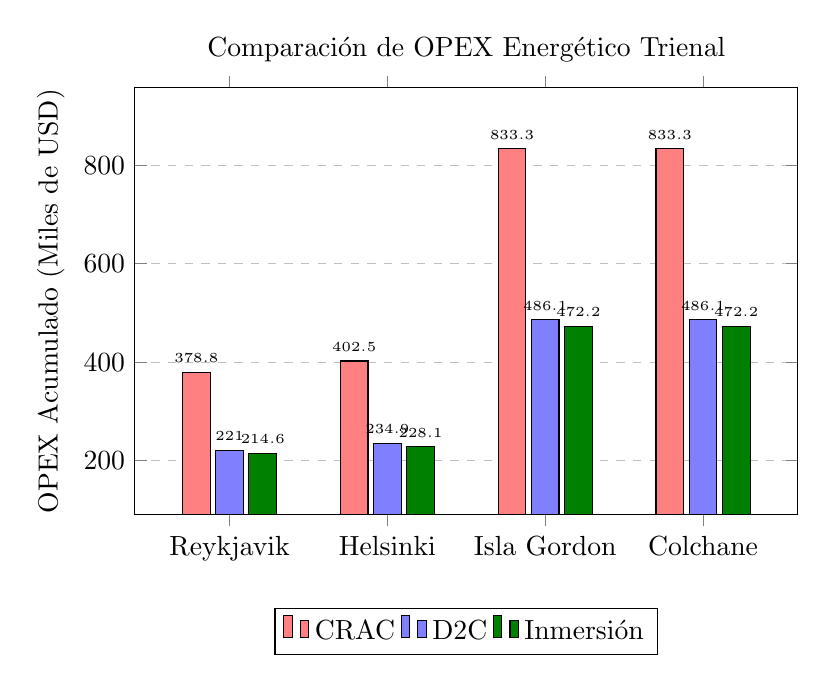
\begin{tikzpicture}
\begin{axis}[
    ybar,
    enlargelimits=0.2,
    legend style={at={(0.5,-0.22)},
      anchor=north,legend columns=-1},
    ylabel={OPEX Acumulado (Miles de USD)},
    symbolic x coords={Reykjavik, Helsinki, Isla Gordon, Colchane},
    xtick=data,
    nodes near coords,
    nodes near coords align={vertical},
    every node near coord/.append style={font=\tiny},
    width=10cm, height=7.0cm,
    title={Comparaci\'on de OPEX Energ\'etico Trienal},
    ymajorgrids=true,
    grid style=dashed
]
% CRAC
\addplot[fill=red!50, draw=black] coordinates {(Reykjavik,378.8) (Helsinki,402.5) (Isla Gordon,833.3) (Colchane,833.3)};
\addlegendentry{CRAC}

% D2C
\addplot[fill=blue!50, draw=black] coordinates {(Reykjavik,221.0) (Helsinki,234.9) (Isla Gordon,486.1) (Colchane,486.1)};
\addlegendentry{D2C}

% Immersion
\addplot[fill=green!50!black, draw=black] coordinates {(Reykjavik,214.6) (Helsinki,228.1) (Isla Gordon,472.2) (Colchane,472.2)};
\addlegendentry{Inmersi\'on}

\end{axis}
\end{tikzpicture}
\caption{Comparativa del costo operativo acumulado (Miles de USD) por localidad y tecnolog\'ia (Fuente: Elaboraci\'on propia).}
\label{fig:opex_bar_chart}
\end{figure}

\section{El trade-off termoecon\'omico: clima vs. tarifa}
El an\'alisis econ\'omico expone una paradoja crucial para la geolocalizaci\'on de data centers: la alta eficiencia t\'ermica de Chile se ve contrarrestada por sus tarifas energ\'eticas industriales \cite{bnef2024}.

La eficiencia econ\'omica ($\eta_{\text{economica}}$) de la transici\'on de CRAC a D2C es equivalente en Isla Gordon e Islandia ($41,7\%$), dado el $100\%$ de Free Cooling logrado en ambas. Sin embargo, el diferencial de costo nominal absoluto es significativo \cite{greenberg2006}:
\begin{equation}
OPEX_{\text{IG}} - OPEX_{\text{R}} = 486.097 - 220.953 = 265.144 \text{ USD}
\end{equation}
Las tarifas el\'ectricas industriales de Chile ($\approx 0,176\text{ USD/kWh}$) duplican a las de las regiones n\'ordicas ($\approx 0,08 - 0,10\text{ USD/kWh}$), lo que hace que la viabilidad comercial en el Cono Sur dependa de contratos preferenciales de compra de energ\'ia limpia (PPAs), la priorizaci\'on de la reducci\'on de huella h\'idrica (cero consumo en Free Cooling seco) y la reducci\'on de latencia de red \cite{bnef2024}.

\section{Optimizaci\'on predictiva con BigQuery ML y Vertex AI}
El modelo de series de tiempo \texttt{ARIMA\_PLUS} en BigQuery ML, entrenado seg\'un la metodolog\'ia descrita en la Sec.~\ref{sec:modelo_arima}, gener\'o un pron\'ostico horariode temperatura de $24\text{ horas}$ para el d\'ia $2026-06-21$ \cite{box2015}, \cite{google2023} (Tabla~\ref{tab:forecast_tesis}).

\begin{table}[htbp]
\caption{Resultados del Pron\'ostico de Temperatura (2026-06-21)}
\label{tab:forecast_tesis}
\centering
\resizebox{\textwidth}{!}{%
\begin{tabular}{lccc}
\toprule
Localidad & Temp. M\'inima ($^\circ\text{C}$) & Temp. M\'axima ($^\circ\text{C}$) & Error Est\'andar ($^\circ\text{C}$) \\
\midrule
Isla Gordon, Chile & $2,18$ & $2,70$ & $1,46$ \\
Colchane, Chile & $6,01$ & $9,30$ & $1,34$ \\
Reykjavik, Islandia & $10,46$ & $11,70$ & $1,28$ \\
Lule\aa, Suecia & $15,85$ & $17,32$ & $1,61$ \\
Helsinki, Finlandia & $17,94$ & $19,93$ & $1,39$ \\
Quebec, Canad\'a & $18,72$ & $20,51$ & $2,09$ \\
\bottomrule
\end{tabular}%
}
\end{table}

Este pron\'ostico se almacena en el esquema relacional de la Sec.~\ref{sec:esquema_bigquery} y se emplea en el sistema BMS para:
\begin{itemize}
    \item \textbf{Control de Caudal Proactivo:} Modula preventivamente la velocidad de los ventiladores y el caudal secundario en el condensador del termosif\'on para mitigar la inercia t\'ermica del bucle de cambio de fase.
    \item \textbf{Planificaci\'on Din\'amica de Tareas (IA):} Si el pron\'ostico muestra temperaturas cercanas al umbral de diseño ($25,0^\circ\text{C}$), se pueden migrar din\'amicamente cargas computacionales de IA hacia locaciones m\'as fr\'ias (ej. migrar tareas de Quebec a Isla Gordon) para evitar el encendido de chillers mec\'anicos y proteger los chips Blackwell \cite{google2014}, \cite{bhardwaj2021}.
\end{itemize}
